\documentclass[10pt,twocolumn,letterpaper]{article}

\usepackage{cvpr}
\usepackage{times}
\usepackage{epsfig}
\usepackage{graphicx}
\usepackage{amsmath}
\usepackage{amssymb}

% Include other packages here, before hyperref.

% If you comment hyperref and then uncomment it, you should delete
% egpaper.aux before re-running latex.  (Or just hit 'q' on the first latex
% run, let it finish, and you should be clear).
\usepackage[breaklinks=true,bookmarks=false]{hyperref}

\cvprfinalcopy % *** Uncomment this line for the final submission

\def\cvprPaperID{****} % *** Enter the CVPR Paper ID here
\def\httilde{\mbox{\tt\raisebox{-.5ex}{\symbol{126}}}}

% Pages are numbered in submission mode, and unnumbered in camera-ready
%\ifcvprfinal\pagestyle{empty}\fi
\setcounter{page}{1}
\begin{document}

%%%%%%%%% TITLE
\title{A Review and Comparison of Boosting Methods}
\author{
Tayler Pauls\\
{\tt\small tayler@bu.edu}
\and
Shen Shen\\
{\tt\small shs2016f@bu.edu}
\and
Alexander Oleinik \\
{\tt\small alxndr@bu.edu}
}
\maketitle
%\thispagestyle{empty}

%%%%%%%%% ABSTRACT
\begin{abstract}
   A thorough review of published boosting methods is performed. Detail and comparison of two Boosting Methods - AdaBoost and Gradient Boosting is described. To outline the impact of these differences, empirical comparisons are performed on multiple datasets to demonstrate their effect on performance. Artificial data was generated to illustrate the effects of noise on boosting performance and examine overfitting-risks associate with boosting methods.  Additionally,  boosting is applied to a real-world application datasets. Performance metrics of AdaBoost and Gradient Boost range in the ninetys, while avoiding overfitting generated and real-world data sets.
 
\end{abstract}

%%%%%%%%% BODY TEXT
\section{Introduction and Review of Literature}
\indent \indent Boosting algorithms are a family of machine-learning ensemble approaches that turn weak classifiers into strong classifiers; they improve classifiers that only outperform random predictions by a small amount. In 1990, Robert Schapire formulated a rigorous explanation of why boosting is possible, He and Yoav Freund pioneered the first practical boosting algorithm - AdaBoost. Although AdaBoost remains popular, there has been significant innovation in the field of Boosting since 1997. Our project dissects the theoretical differences among Boosting algorithms and provide empirical results to depict data-set categories where particular Boosting methods excel. 
 
In our review of literature, we examined original literature describing AdaBoost and Gradient Boost methods \cite{schapire2012boosting} \cite{schapire1999improved} \cite{friedman2001greedy} as well as the effects of noise on various boosting methods \cite{long2010random}

%-------------------------------------------------------------------------
\section{Model}
\indent \indent The goal of boosting is to generate a strong learner from a set of weak learners. The most popular algorithms, AdaBoost and Gradient Boost, strengthen the learners by using a linear combination of the predictions of the weak learners. In general. given weak classifiers $h_1(x)...h_n(x)$, the prediction is given by:
\begin{equation}
F(x)=\sum_{i=1}^{n}W_ih_i(x)
\end{equation}
\indent Boosting methods vary according to the techniques used to learn the weights $W_i$. Additionally, boosting algorithms are often coupled with various strategies for obtaining the weak learners $h_i(x)$. Gradient Boost is an example of such a greedy method where the weak learners are usually generated iteratively.
%-------------------------------------------------------------------------
\subsection{AdaBoost}
\indent  AdaBoost is a binary classification model that combines several weak learners and combines them linearly to form a strong classifier. The weak classifiers are given to the AdaBoost model, and AdaBoost weights them based on their performance of reducing the error. In AdaBoost, each learner is initially assigned and equally weighted. The weights are iteratively updated to reflect the relative performance of each classifier to maximize the overall performance. AdaBoost can use any weak classifiers to learn from, but they must be assigned initially.  The weak learners used in this application of AdaBoost are single-split decision trees, known as \textit{"Decision Stumps"}. 

\subsubsection{Loss Function and $\alpha$}
\indent  Given a data set ${(x_1,y_1)...(x_n,y_n)}$ and weak classifiers $h_1(x)...h_t(x)$ , the objective of adaboost is to assign weights, $\alpha_t$, to the weak classifiers to minimize the exponential loss function, E:
\begin{equation}
E = \sum_{i=1}^{n}\exp(-y_i*F_t(x_i))
\end{equation}
where $F_t(x_i)$ is defined as:
\begin{equation}
F_t(x_i) = F_{(t-1)}(x_i)+\alpha_t*h_t(x_i)
\end{equation}
$\alpha_t$ is assigned weight for particular weak classifier
\cite{adaorig}

\indent The first term in $F_t(x_i) $ is the previous combination of weighted classifiers from all previous weak classifiers, and is constant. Therefore, we can rewrite the loss function as:
\begin{equation}
E = \sum_{i=1}^{n}\exp(-y_i*(F_{(t-1)}(x_i))*\exp(F_t(x_i)))
\end{equation}
assigning $\exp(F_{(t-1)}(x_i))$ as $\omega_i^{t}$,
the loss function becomes:
\begin{equation}
E = \sum_{i=1}^{n}\omega_i^{t}*\exp(-y_i*\alpha_t*h_t(x_i))
\end{equation}
\indent Since AdaBoost is a binary classifier, the inside of the exponent will be positive if the ground truth, $y_t$, and the weak classifier, $h_t(x_i)$, agree (correct classification), and negative if they don't agree (incorrect classification). Therefore, we can separate out the exponentials in the loss function based on correct(first $\sum$), and incorrect classification(second $\sum$):
\begin{equation}
E = \sum_{i=1}^{n}\omega_i^{t}*\exp(\alpha_t) +  \sum_{i=1}^{n}\omega_i^{t}*\exp(-\alpha_t)
\end{equation}
Setting the derivative with respect to $\alpha$ and setting it to zero will yield an expression for $\alpha$ that minimizes total error since the error function is convex.
\begin{equation}
\frac{\partial E}{\partial \alpha_t}=0 = \frac{\partial (\sum_{i=1}^{n}\omega_i^{t}*\exp(\alpha_t) +  \sum_{i=1}^{n}\omega_i^{t}*\exp(-\alpha_t))}{\partial \alpha_t} 
\end{equation}
solving for $\alpha_t$ yields\cite{schapire1999improved}:
\begin{equation}
\alpha_t = 0.5\log\left(\frac{\sum_{y_i=h_t(x_i)} \omega_i^{t}}{\sum_{y_i \ne h_t(x_i)} \omega_i^{t}}\right)
\end{equation}
as a shortcut, $\sum_{y_i \ne h_t(x_i)} \omega_i^{t} = \epsilon$,
and $\sum_{y_i = h_t(x_i)} \omega_i^{t} = 1-\epsilon$

\subsubsection{Algorithm \cite{adalecture}}
\textbf{input}: classifiers $h_1(x)...h_t(x)$, training data ${(x_1,y_1)...(x_n,y_n)}$ 
\begin{enumerate}
\item Set weights $W_i = \frac{1}{n}$
\item For $t=1...num_classifiers$
\begin{enumerate}
\item Calculate the weighted error of $h_t$ over the training data. For:
$ h_t(x_i)\ne y_i$
\begin{equation}
\epsilon_t = \sum_{i=1}^{n}W_i 
\end{equation}
\item Compute $\alpha$
\begin{equation}
\alpha_t = 0.5\log\left(\frac{1-\epsilon_t}{\epsilon_t}\right)
\end{equation}
\item Update Weights 
\begin{equation}
W_i,t+1=\frac{W_i,t}{b}*\exp(-y_i\alpha_th_t(x_i))
\end{equation}
$b$ is chosen such that $\sum W_i = 1$
\end{enumerate}
\end{enumerate}
\paragraph{Properties} As the number of iterations and weak classifiers increases, the exponential loss of the cumulative classifier over the training set strictly decreases.

\subsubsection{Decision Stumps}
Although, the core of AdaBoost is independent of the weak classifiers, in practice the generation of these learners is combined with the boosting procedure. For this application of AdaBoost, the weak classifiers are stumps generated with a decision tree learning method. There are many such methods - some common strategies are outlined below:
\begin{itemize}
\item For individual features, locate sets where there is a perfect split between classes, like figure \ref{fig:stump1}.

\begin{figure}[h!]
  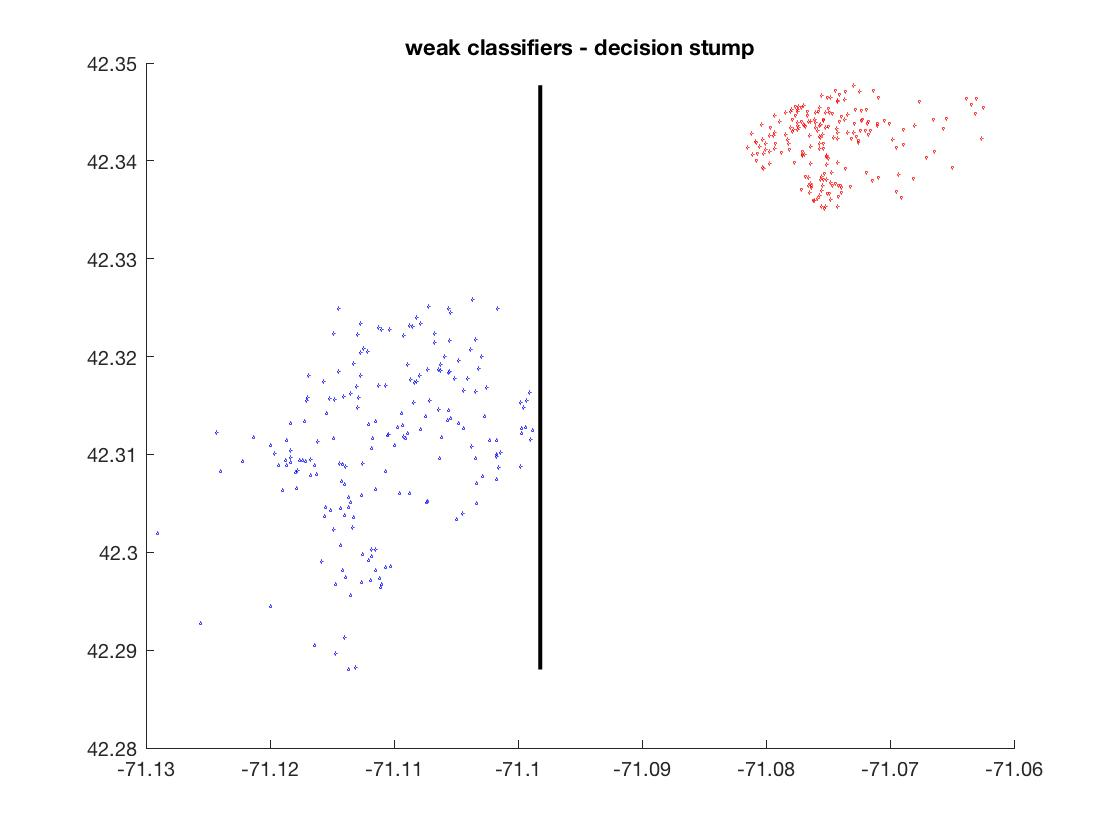
\includegraphics[width=\linewidth]{decisionstump_1.jpg}
  \caption{perfectly separated by 1 decision stump.}
  \label{fig:stump1}
\end{figure}

\item For relatively small data sets, iterate over all possible unique binary separations in each feature's space, and analyze the performance of each as a classifier. For example, Figure \ref{fig:stump2} combines three decision stumps to classify.
\begin{figure}[h!]
  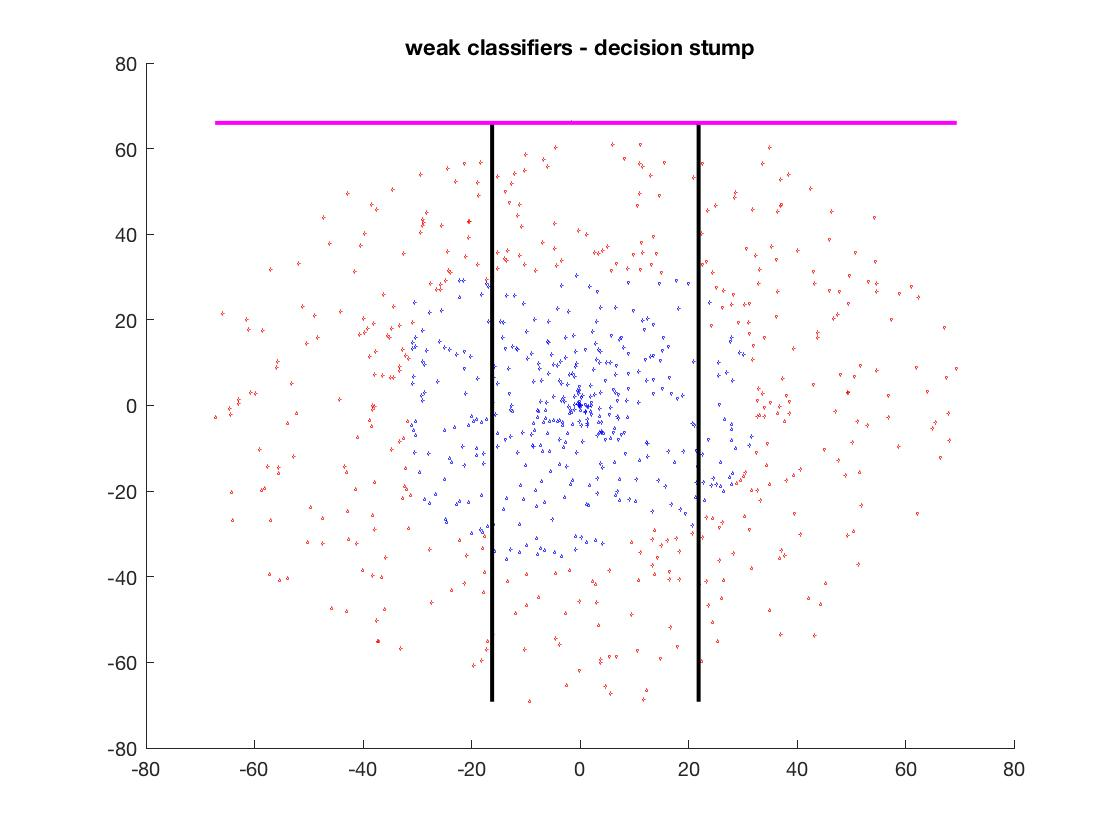
\includegraphics[width=\linewidth]{decsiontree_3.jpg}
  \caption{multiple stumps for more complex data.}
  \label{fig:stump2}
\end{figure}
\end{itemize}

%-------------------------------------------------------------------------
\subsection{Gradient Boosting}

AdaBoost constructs a strong classifier or regressor from a set of weak basic learners. These learners are provided before the boosting process begins. However, boosting algorithms can also specify the process for generating a new learner. One approach, called Gradient Boosting, iteratively generates weak learners by implementing the gradient of the loss. The following formula is a simple idea of generating a gradient boosting model.

Assume we have a data set 
$\{(\,x_1,y_1)\,...(\,x_n,y_n)\,\}$, where for each sample $x_i\in \mathbb {R}^d$ has a label $y$. Similar to AdaBoost, we generate the model as:
\begin{equation} F(x) = \sum_{i=1}^{M} f_m(x_i) = F_{m-1}(x_i) + f_m(x_i) \end{equation}

Our object is to find the $f_m(x)$ to minimize the loss $\mathbb {L}$. 
The first step of gradient boosting is to initialize the model with a very simple learner. By doing prediction only based on the mean or mode of the ground truth label, generally, this model only has one parameter $\gamma_0$, so the initialization could be written as:
\begin{equation}f_0(x) = \underset{\gamma_0}{\arg\min} \sum_{i=1}^n L(y_i, \gamma_0) \end{equation}

In order to build a new learner that can minimize the loss in next step, we want
\begin{equation}
f_m(x) = \underset{fm}{\arg\min} \sum_{i=1}^n L(y_i, F_{m-1}(x_i)+f_m(x_i))
\end{equation}
In most cases, identifying the optimal function $f_m(x)$ at each step is computationally impossible. As with other optimization problems, we apply a gradient descent and greedy criterion as an approximation. Suppose that
\begin{equation}
f_m(x) = \gamma_m h_m(x)
\end{equation}

Where $\gamma_m$ is the step length of the gradient decent algorithm and $h_m(x)$ is the weak learner we build to fit in the gradient of the loss to our current model. This gradient is called the pseudo-residual $r_m$:
\begin{equation}
r_m = -\frac{\partial L(y,F(x)}{\partial F(x)} |_{F(x)=F_{m-1}(x)} 
\end{equation}

Instead of using a fixed step length for every iteration, Gradient boosting calculates an adaptive step length $\gamma_m$ to minimize the loss given $h_m(x)$.
\begin{equation}
\gamma_m = \underset{\gamma}{\arg\min} \sum_{i=1}^n L(y_i,F_{m-1}(x_i)+\gamma r_m)
\end{equation}

The value of $\gamma_m$ can be calculated by line searching from the above equations.

\subsubsection{Algorithm}
\textbf{input}: training data ${(x_1,y_1)...(x_n,y_n)}$ 
\begin{enumerate}
\item Initialize  $F_0(x) = \underset{\gamma_0}{\arg\min} \sum_{i=1}^n L(y_i, \gamma_0)$
\item For $m=1$...max iteration
\begin{enumerate}
\item Calculate the pseudo-residuals
\begin{equation}
r_m = -\frac{\partial L(y,F(x)}{\partial F(x)} |_{F(x)=F_{m-1}(x)} 
\end{equation}
\item Find a weak learner $h_m(x)$ to fit in $r_m$
\item Calculate the adaptive step length $\gamma_m$
\begin{equation}
\gamma_m = \underset{\gamma}{\arg\min} \sum_{i=1}^n L(y_i,F_{m-1}(x_i)+\gamma r_m)
\end{equation}
\item Update the model:
\begin{equation}
F_m = F_{m-1}(x)+\gamma_m h_m(x)
\end{equation}

\end{enumerate}
\end{enumerate}
\subsubsection{Shrinkage}
When the max number of iterations grow, severe overfitting can harm the behavior of the gradient model. One way to reduce this impact is to modify the model by adding a shrinkage parameter, $\nu$ such that $0<\nu<1$, that decreases the step length at each iteration. By taking this modification, the updated function can be rewritten as $F_m = F_{m-1}(x)+\nu\gamma_m h_m(x)$. This "shrinkage parameter" is also called the learning rate.

\section{Results}
\subsection{AdaBoost}
An AdaBoost function created by Dr. Kroone from University of Twente was modified in MATLAB and used in the main AdaBoost implementation. Fifty decision stumps were used for classification, half horizontal and half vertical. Data was generated or gathered for the following AdaBoost Applications: Toy problem and Boston Neighborhood Classification. 

\subsubsection{Toy Problem}
One thousand Random sin/cosine angle data points were generated for this toy problem to create x,y locations so that class one is a small circle and class two is a larger ring outside of class one, depicted in figure \ref{fig:ada1}. The entire dataset was partitioned into training and testing sets for classification. $80\%$ were used as the training set and remaining $20\%$ used for testing. 
\begin{figure}[h!]
  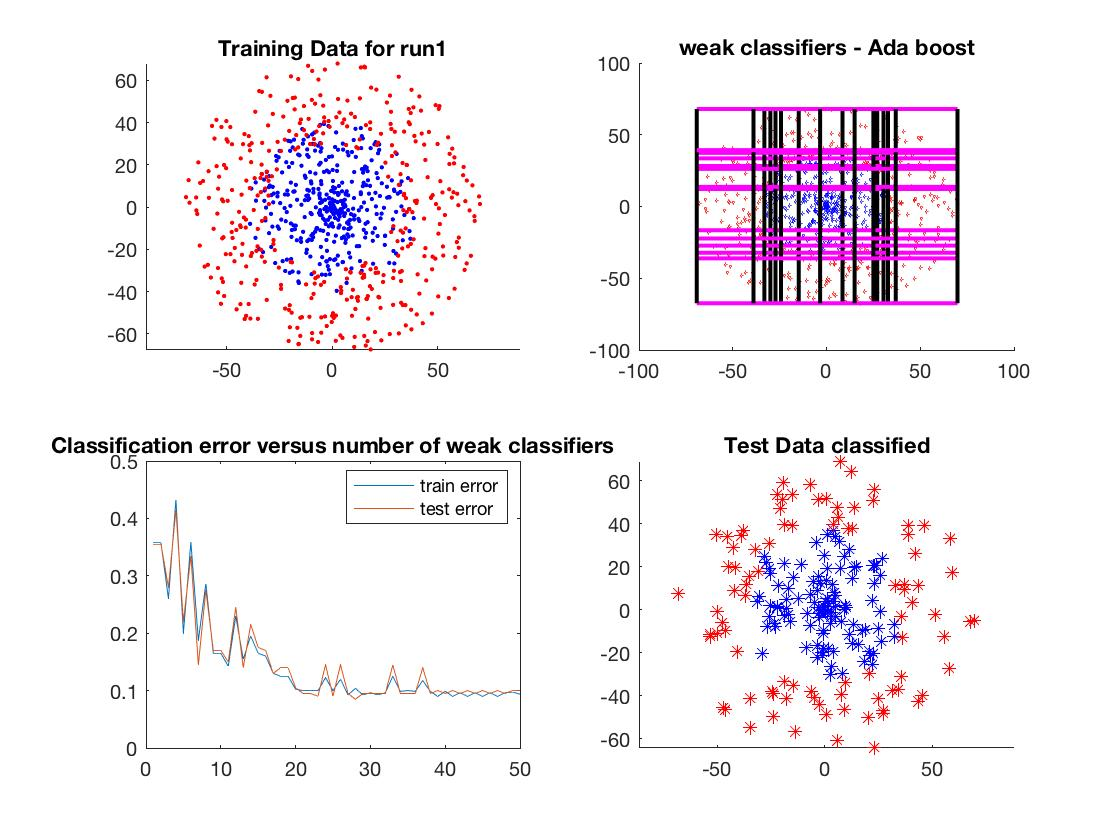
\includegraphics[width=\linewidth]{ada_fig1.jpg}
  \caption{AdaBoost for a Toy Example}
  \label{fig:ada1}
\end{figure}

\indent It is clear from the bottom left image in figure \ref{fig:ada1} that the training error is indeed bounded by an exponential function. Another important conclusion by looking at the testing error in bottom left in figure \ref{fig:ada1} is that AdaBoost does not overfit.  Finally,  Adaboost seperates the data well geometrically, illustrated in the top right image in figure \ref{fig:ada1}.

\subsubsection{Boston Neighborhood Classification}

Boston Neighborhood data was obtained from
\url{http://insideairbnb.com/get-the-data.html}. This dataset is 2558 houses listed on Airbnb in the Boston area for October 2015. From the entire data set of neighborhoods, the top five neighborhoods with the largest amount of data-points were selected for classification.  Four separate classifications were performed: one-vs-one AdaBoost, one-vs-all AdaBoost, linear SVM, and RBF SVM with a Gaussian kernel.  The figures show an OVO- AdaBoost example,figure \ref{fig:ada2}, and an OVA-AdaBoost example,figure \ref{fig:ada3}. Just like the toy problem, the model does not overfit the data and performs well. 

\begin{figure}[h!]
  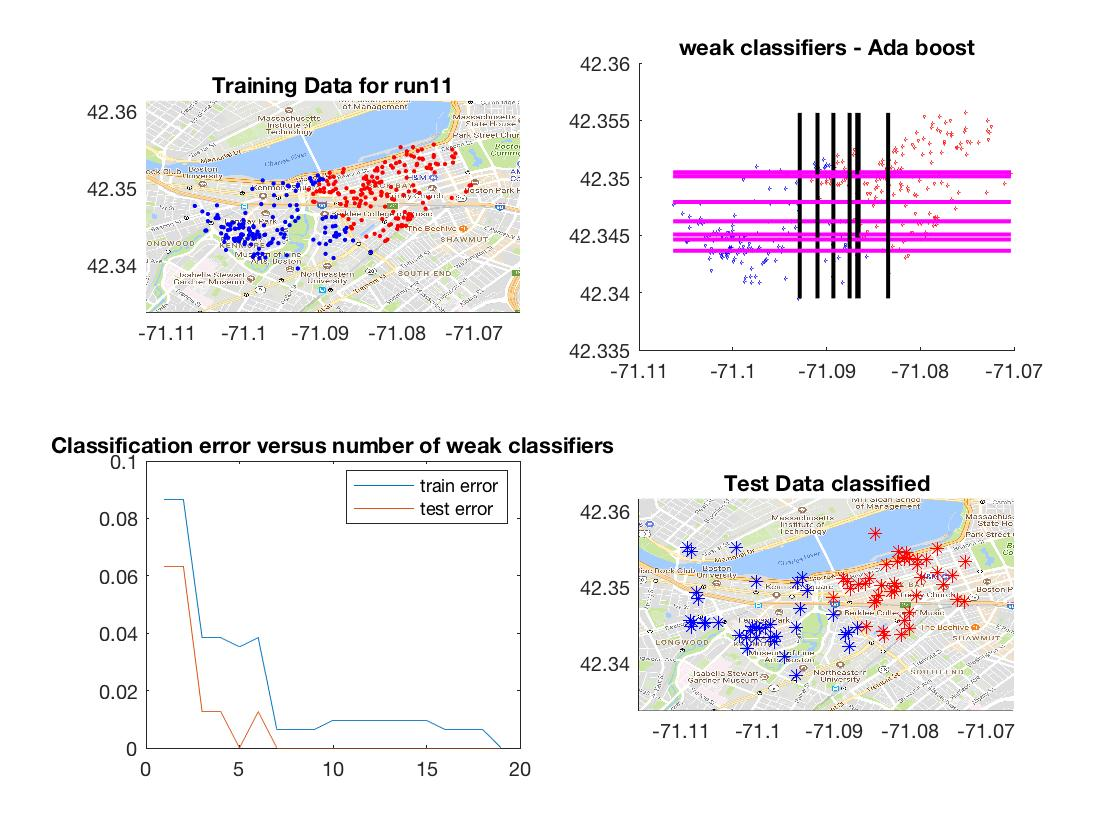
\includegraphics[width=\linewidth]{ada_fig2.jpg}
  \caption{AdaBoost OVO.}
  \label{fig:ada2}
\end{figure}

\begin{figure}[h!]
  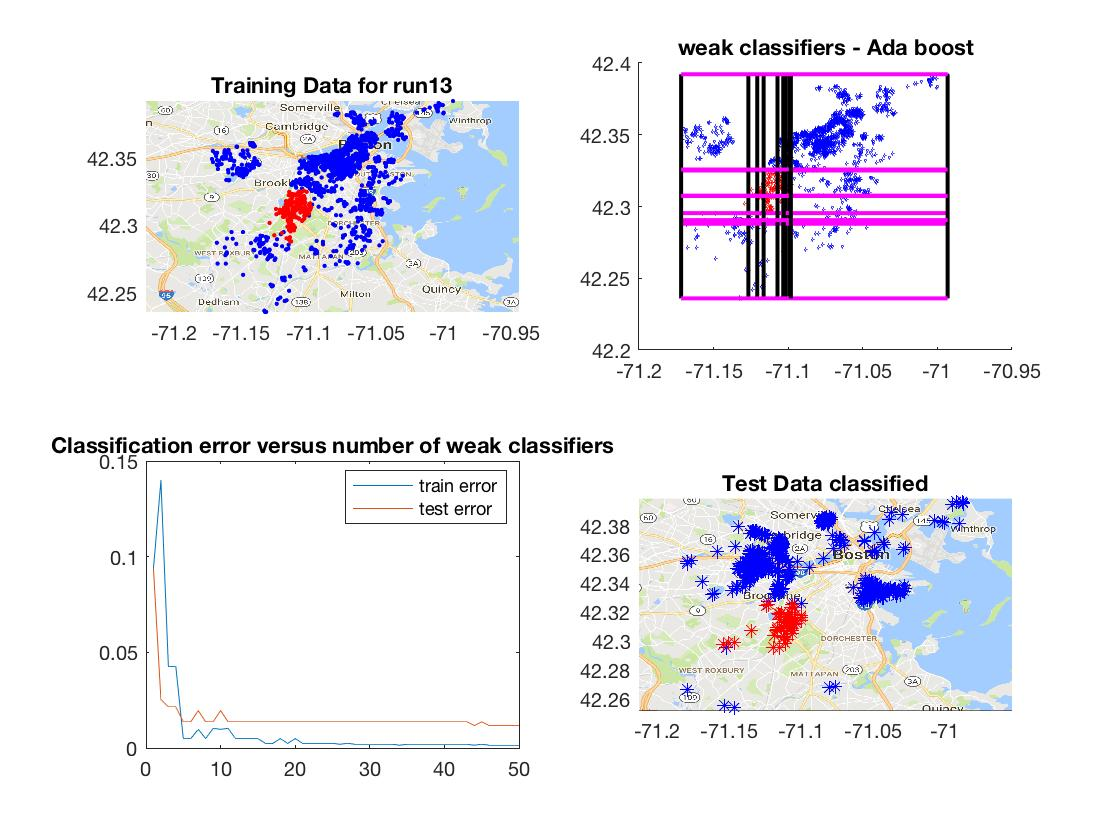
\includegraphics[width=\linewidth]{ada_fig3.jpg}
  \caption{AdaBoost OVA.}
  \label{fig:ada3}
\end{figure}

\indent Linear SVM performs very poorly, and rbf-SVM performs very well.  The box constraint and sigma value for RBF-SVM were chosen through an exhaustive grid-search to find where the maximum CCR would occur based on the dataset. Table \ref{table:adaccr} shows the CCR values of each different run conducted on this dataset. \\

\begin{table}[ht]
\centering
\caption{Adaboost vs SVM CCR}
 \begin{tabular}{||c c c c||} 
 \hline
  & min-ccr & mean-ccr & max-ccr \\ 
 \hline\hline
AdaBoost, OVO & 98.661 & 96.471 & 100  \\ 
 \hline\hline
AdaBoost, OVA &96.052 & 87.524 & 99.609 \\ 
\hline\hline
SVM - linear & 44.854 & 9.9415 & 81.641 \\ 
\hline\hline
SVM - rbf & 99.561 & 99.414 & 99.61 \\
C = 512 $\sigma = 0.0078$ & & & \\
 \hline \hline
\end{tabular}
\label{table:adaccr}
\end{table}
\indent Although RBF SVM and AdaBoost performance is comparable, AdaBoost is less computationally  intensive, and performed faster. For this use case, it outperformed RBF SVM by all metrics.

\subsection{Gradient Boosting}
 We apply the Gradient Boosting method on the Boston house-price dataset \url{http://lib.stat.cmu.edu/datasets/boston}. In this data set, there are 14 features, such as town crime rate, which are used to predict the house price. The dataset provides a total of 506 samples. For implementing the Gradient Boosting model, 90\% of the data will be separated as training data and the others are the testing data. 10-fold cross-validation is performed. Our goal is to compare the Gradient Boosting performance for fixed, adaptive and "shrinkage" step lengths. Additionally, we examine the performance of the model on complex regressors as the basic learners. 

\subsubsection{Step length}

Gradient Boosting model is tested with different step lengths. The loss function in the demonstration is MSE loss. Notation iter indicates how many basic learners the gradient boost model uses. The basic learner here is CART regression trees with max depth 2. Step length is fixed to 0.1 and shrinkage parameter is 0.05.

\begin{table}[ht]
\centering
\caption{Performance of gradient boosting with tree depth = 2}
 \begin{tabular}{||c c c c c||} 
 \hline
iter & step length & final tr-loss & final ts-loss & min ts-loss \\ 
 \hline\hline
20   & fix(0.1) & 2.368 & 11.086 & 11.086  \\ 
 \hline\hline
20   & adapt & 4.544 & 8.499 & 7.908 \\ 
\hline\hline
200  & adapt & 0.043 & 8.681 & 7.187 \\ 
\hline\hline
200  & shrink & 4.504 & 6.416 & 6.416\\ 
 \hline\hline
\end{tabular}
\label{table:d2gbloss}
\end{table}

\begin{figure}[h!]
  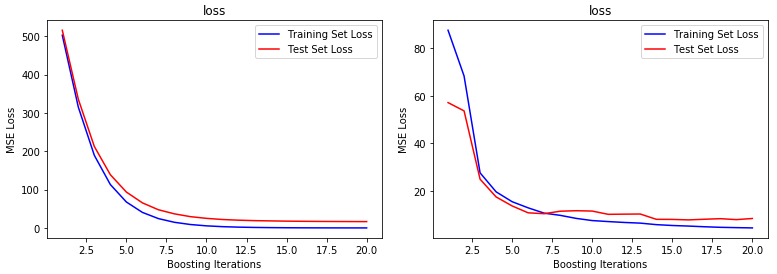
\includegraphics[width=\linewidth]{fixsl20.png}
  \caption{20 iterations with fix and adaptive step length}
  \label{fig:gb1}
\end{figure}
\begin{figure}[h!]
  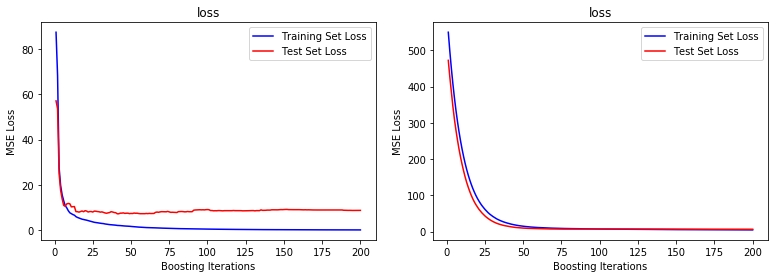
\includegraphics[width=\linewidth]{adaptsl200.png}
  \caption{200 iterations with adaptive and shrinkage step length}
  \label{fig:gb2}
\end{figure}
Figure \ref{fig:gb1} reveals how adaptive step length affects the performance of the Gradient Boosting model. Compared with fixed step length, adaptive step length reaches lower test loss. The reason is that it reasonably chooses the weight of each basic learner.\\
Figure \ref{fig:gb2} shows that continually adding basic learners causes overfitting. Shrinkage learning rate reduces the overfitting effect and improves the generalization ability of the model.\\
\subsubsection{Basic learners}
The following experiment is to test the performance of Gradient Boosting model by choosing different basic learners. The basic learner here is CART regression trees with max depth 8.

\begin{table}[ht]
\centering
\caption{performance of gradient boosting with tree depth = 8}
 \begin{tabular}{||c c c c c||} 
 \hline
iter & step length & final tr-loss & final ts-loss & min ts-loss \\ 
 \hline\hline
20   & fix(0.1) & 7.4e-2 & 11.031 & 15.360  \\ 
 \hline\hline
20   & adapt & 8.4e-5 & 26.10 & 24.39 \\ 
\hline\hline
200  & adapt & 0 & 27.77 & 26.700 \\ 
\hline\hline
200  & shrink & 1.2e-3 & 10.614 & 10.052\\ 
 \hline\hline
\end{tabular}
\label{table:d8gbloss}
\end{table}
\begin{figure}[h!]
  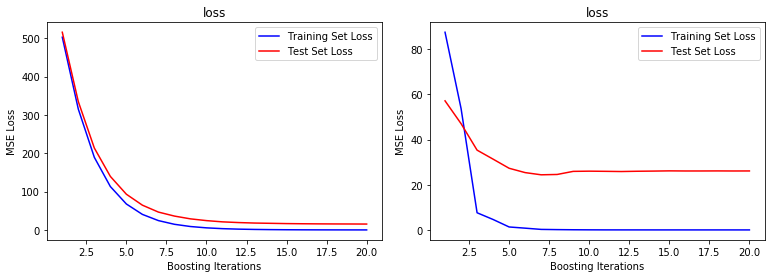
\includegraphics[width=\linewidth]{a.png}
  \caption{20 iterations with fix and adaptive step length}
  \label{fig:gb3}
\end{figure}
\begin{figure}[h!]
  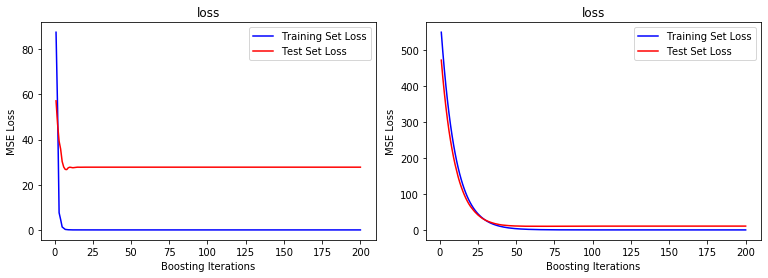
\includegraphics[width=\linewidth]{c.png}
  \caption{200 iterations with adaptive and shrinkage step length}
  \label{fig:gb4}
\end{figure}

The comparison result shows that implementing a stronger basic learner can reduce the training loss to near zero but significantly harms the generalization ability. Even though we implement a shrinkage learning rate, the performance of the model is not as good as using a weaker basic learner.\\

\section{Comparison of Boosting Methods}
The examples detailed above illustrate the differences between AdaBoost and Gradient boost.  It is impossible to make strong general conclusions about these methods simply by performing their performance for specific datasets. The fundamental differences such as weak learner source and number of parameters make extrapolating from a unrelated couple datasets impossible. Instead we examine their performance, independently, while methodically modifying a dataset.     
\subsection{Salt and Pepper Noise}
One common application of Boosting is character recognition. We examine the performance of Boosting as we add noise to the MNIST character dataset. We add salt and pepper noise, which replaces certain features/pixels with white or black at a configured rate.
\begin{figure}[h!]
  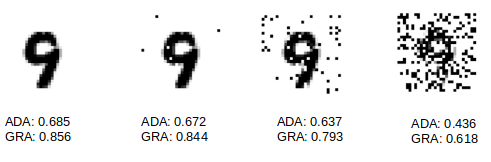
\includegraphics[width=\linewidth]{fig1.png}
  \caption{AdaBoost and Gradient Boost performance at 0\%, 2\%, 6\% and 9\% Noise Levels}
  \label{fig:c1}
\end{figure}
\begin{figure}[h!]
  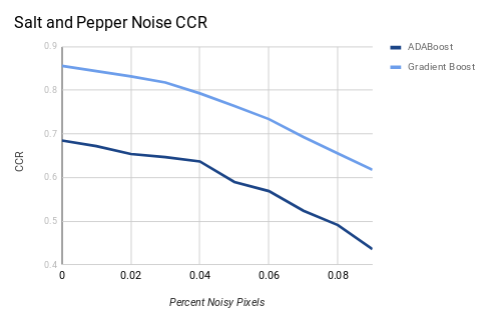
\includegraphics[width=\linewidth]{fig2.png}
  \caption{AdaBoost and Gradient Boost performance vs Noise Level}
  \label{fig:c2}
\end{figure}
These results are inconclusive. There seems to be no obvious performance difference between AdaBoost and Gradient Boost with increased noise, for this high-dimensional dataset.  

\subsection{Outliers}
Instead of adding salt and pepper noise to the features of the MNIST data, we create outliers by replacing labels at random with an increasing rate.
\begin{figure}[h!]
  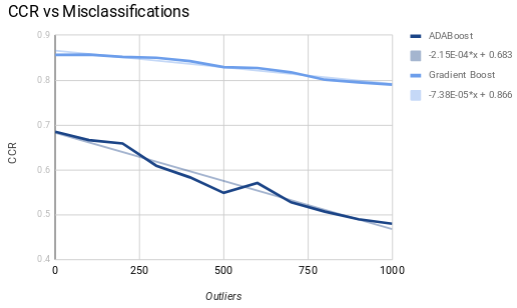
\includegraphics[width=\linewidth]{fig3.png}
  \caption{AdaBoost and Gradient Boost performance vs Noise Level}
  \label{fig:c2}
\end{figure}
Unlike the previous example, there is an evident difference in the slope of the CCRs as the number of outliers increases. ADABoost is affected more that Gradient Boost.

In order to better visualize this behavior, we create a toy regression dataset of samples selected from a 2-D sinusoidal function applied over a normal curve. The X dimension is selected as the feature and the Y as the label. 80\% of the samples are used to train ADABoost and Gradient Boost learners. We iteratively select sample labels and apply transformations to them to turn them into outliers, by scaling them by negative factors. We test all of the points and draw the results on graphs at each step. 
\begin{figure}[h!]
  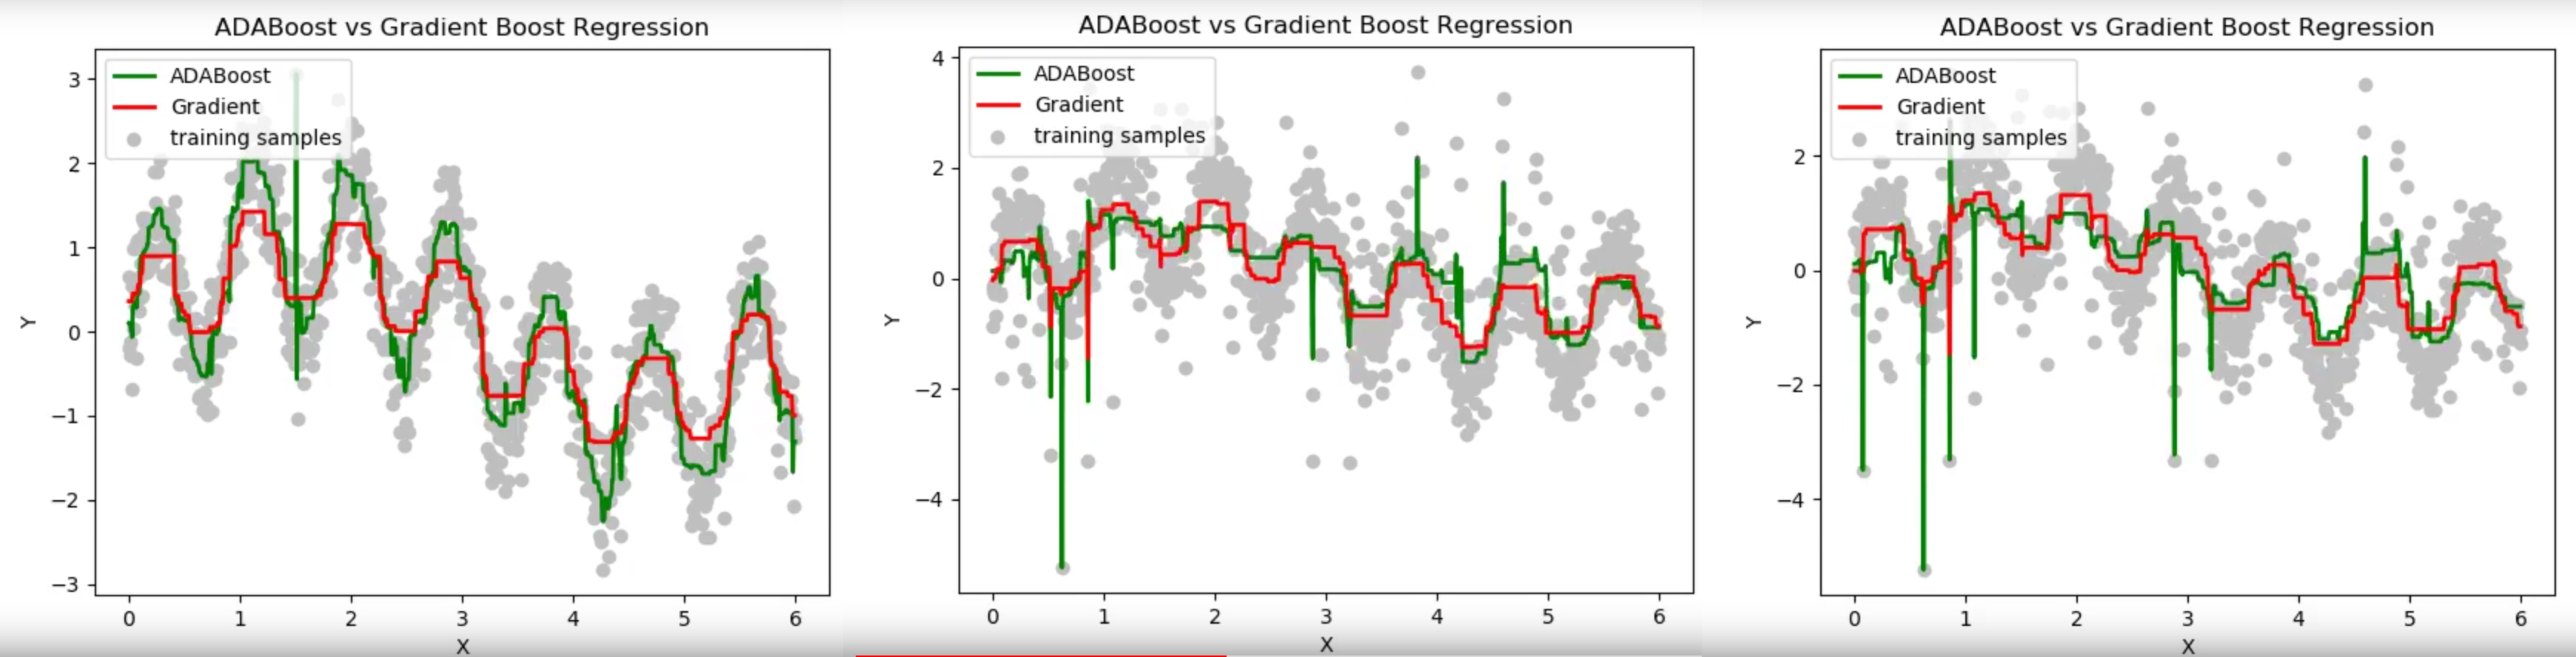
\includegraphics[width=\linewidth]{fig4.png}
  \caption{Samples, and AdaBoost, Gradient Boost predictions at 0 Outliers, 75 outliers and 150 outliers}
  \label{fig:c2}
\end{figure}
This provides a good illustration of results similar to the previous classification problem. AdaBoost immediately begins to fit to certain outliers as seen by the drastic changes to the regression curve. Gradient Boost does not suffer from this issue - it's shape changes naturally as the number of outliers increases, but few outliers have no effect. This is explained by the fact that this application of Gradient Boost uses a Log loss unlike AdaBoost's convex exponential loss function which is susceptible to noise/outliers.
\subsection{A Note about Overfitting} 
In AdaBoost literature, there is mention that boosting methods do not seem to be susceptible to overfitting, as long as learners are kept sufficiently weak. \cite{schapire2012boosting} The consequences of using strong-learners are illustrated in the Gradient Boost section, but we attempt to reconcile this with the results from the toy-regression problem above. If AdaBoost is susceptible to individual outliers, how can it not overfit? The answer to this question lies in the fact that only a small fraction of the feature space is affected by the major outlier "trenches". At 150-200 outliers, on average only \%0.09 of the feature space deviated significantly from neighboring predictions at a \%0.005 resolution. Thus, even if AdaBoost can drastically compensate for individual outliers, this should not have a significant affect associated with over-fitting during the testing stage. 

\section{Conclusion}
Boosting is a sort of supervised machine learning methods that ensemble basic learner as a strong classifier or regressor. The methods compared are Adaboost, which combines given weak learners, and Gradient Boosting, which generates weak learners through learning.

We implement Adaboost to solve a multi-class classification problem by OVO and OVA model and compare it with lineal and kernel SVM. The result shows that Adaboost can achieve comparable good performance as kernel SVM with less computational intensity. Then we implement Gradient boosting on a house price regression problem. The result shows that Gradient Boosting achieves relatively accurate prediction with weak basic learners. More iterations with shrinkage learning rate can help improve the performance.

Finally we tested noise and outliers and found the affects of Adaboost and Gradient Boosting. 

\subsection{Division of Labor}
The team collaborated on each aspect of the project, with each member focusing on a method or procedure. There is an even $\%33\frac{1}{3}$ split in labor among the team members.
\begin{itemize}
\item   Tayler tests Adaboost classification ability by visualize weak decision stumps in low-dimension feature spaces
\item   Shen generates simple Gradient boosting Class and test its performance by tuning the model
\item   Alex compares Adaboost and Gradient Boosting to data with noise and outliers
\end{itemize}

\bibliography{bib.bib}
\bibliographystyle{plain}

\nocite{*}
\end{document}
